\documentclass[11pt]{homework}

\usepackage[UTF8]{ctex}
\usepackage{graphicx}
\usepackage{float} 
\usepackage{subfigure}
\usepackage{listings}
\lstset{breaklines=true}

\newcommand{\hwname}{封钰震}
\newcommand{\hwemail}{1951362}
\newcommand{\hwtype}{作业}
\newcommand{\hwnum}{0-词法分析器}
\newcommand{\hwclass}{Java语言程序设计}
\newcommand{\hwlecture}{}
\newcommand{\hwsection}{}

\usepackage{lipsum}

\begin{document}
\maketitle

\question*{编程环境}

  \subsection*{硬件环境}
  \begin{enumerate}
    \item 型号名称:MacBook Pro
    \item 处理器名称:Dual-Core Intel Core i5
    \item 内存:8 GB
  \end{enumerate}

  \subsection*{软件环境}

  系统版本:macOS 10.15.7 (19H1030)

  \subsection*{运行环境}

  \begin{enumerate}
    \item C++ Language Dialect: GNU++14[-std=gnu++14]
    \item C++ Standard Library: libc++
  \end{enumerate}

\question*{设计思想}

  \subsection*{关键算法}

  编译器进行词法分析时会使用一些字符串匹配算法,常见的字符串匹配算法包括:朴素字符串匹配算法、Radin-Karp算法、利用有限自动机进行字符串匹配、Knuth-Morris-Pratt算法。这些字符串匹配算法的最坏时间复杂度均是线性的。本次作业中的算法是基于朴素字符串匹配算法进行的改变。

  \subsubsection*{朴素字符串匹配算法}

  对于已知的待匹配字符串$T[1, \cdots, n]$和匹配的模式$P[1, \cdots, m]$,朴素字符串匹配算法是利用一次遍历,寻找到待匹配字符串中的位置$s$,使得$P[1, \cdots, m] = T[s+1, \cdots, s+m]$,算法的示意图如图\ref{naive-matching-algorithm}所示。

  \begin{figure}
    \centering
    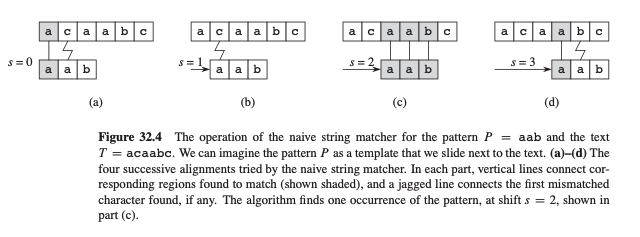
\includegraphics[width=\textwidth]{naive-matching-algorithm}
    \caption{朴素字符串匹配算法}
    \label{naive-matching-algorithm}
  \end{figure}

  本次作业中基于朴素字符串匹配算法的实现具体可见下一节“判断依据”中的分析。

  \subsection*{判断依据}

  本程序打开目标文件后逐行读取,读取后调用函数$lexicalAnalyse$、逐行进行判断。

  函数$lexicalAnalyse$中有一静态变量$is\_in\_comment$,用于表示读取的一行代码是否处在形如
  \lstset{language=c++}
  \begin{lstlisting}
    /*
    comment
    */
  \end{lstlisting}
  的跨行注释中,初始时该静态变量设为$false$。

  若读取的一行代码处在跨行注释中,即$is\_in\_comment = true$,则寻找注释结束的标志“*/”。如果没有找到,则继续读下一行;如果注释结束,则将$is\_in\_comment$设为$false$,并以注释结束处到该行结束处的子串为参数,调用函数$lexicalAnalyse$,调用完成后即可进入下一行的读取、分析。

  若读取的一行代码不处在跨行注释中,即$is\_in\_comment = false$,则此时定义两变量$left = right = 0$,再依次进行下列判断:
  \begin{enumerate}
    \item 是否以‘\#’开头。若是,则为预处理语句,返回(return),进入下一行的分析;
    \lstset{language=c++}
    \begin{lstlisting}
      str[left] == '#'
    \end{lstlisting}
    \item 是否由双引号包裹(需跳过作为转义字符的双引号)。若有,则是字符串常量,$left$与$right$加至字符串后的位置;
    \lstset{language=c++}
    \begin{lstlisting}
      if (str[left] == '"') {
        int i = left + 1;
        for ( ; i < len; i++) {
          if (str[i] == '"' && str[i - 1] != '\\') {
            break;
          }
        }
        // ...
      }
    \end{lstlisting}
    \item 是否有以“/*”开头的注释。若有这样的注释,则在该行寻找“*/”。如果找到了“*/”,则$left$与$right$加至注释后的位置;如果没有找到,则设置$is\_in\_comment = true$,返回;
    \lstset{language=c++}
    \begin{lstlisting}
      if (left < len - 1 && str[left] == '/' && str[left + 1] == '*') {
        int i = left + 2;
        for ( ; i < len - 1; i++) {
          if (str[i] == '*' && str[i + 1] == '/') {
            break;
          }
        }
        // ...
      }
    \end{lstlisting}
    \item 是否有以“//”开头的注释。若有,则返回,进入下一行的分析;
    \lstset{language=c++}
    \begin{lstlisting}
      left < len - 1 && str[left] == '/' && str[left + 1] == '/'
    \end{lstlisting}
    \item 是否由单引号包裹(需跳过作为转义字符单引号)。若有,则是字符常量,$left$与$right$加至字符后的位置;
    \lstset{language=c++}
    \begin{lstlisting}
      if (str[left] == '\'') {
        int i = left + 1;
        for ( ; i < len; i++) {
          if (str[i] == '\'' && str[i - 1] != '\\') {
            break;
          }
        }
        // ...
      }
    \end{lstlisting}
    \item 是否由数字开头,后面紧跟数字、‘e’‘E’‘+’‘-’‘.’等符号;一直遍历,直到遇到不包含在这些之内的字符。$left$与$right$加至在后;
    \lstset{language=c++}
    \begin{lstlisting}
      if (str[left] <= '9' && str[left] >= '0') {
        int i = left + 1;
        for ( ; i < len; i++) {
          if (!((str[i] <= '9' && str[i] >= '0') || str[i] == '.' || str[i] == 'e' || str[i] == 'E' || str[i] == '+' || str[i] == '-')) {
            break;
          }
        }
        // ...
      }
    \end{lstlisting}
    \item 是否$right$处为分隔符。若有,且此时$left = right$,则$left$与$right$加至分隔符后的位置;
    \lstset{language=c++}
    \begin{lstlisting}
      isSeparator(str[right]) == true && left == right
    \end{lstlisting}
    \item 是否$right$处为运算符。若有,且此时$left = right$,则由运算符开始,一直遍历,直到遇到不是运算符的字符,$left$与$right$加至运算符后的位置;
    \lstset{language=c++}
    \begin{lstlisting}
      isOperator(str[right]) == true && left == right
    \end{lstlisting}
    \item 若$right$处的字符不是分隔符,也不是运算符,又由于上面程序对各种特殊字符依次进行了判断,$right$处的字符应是标识符或关键字的一部分。则此时$left$保持不变,将$right$向右移动。
    \lstset{language=c++}
    \begin{lstlisting}
      isSeparator(str[right]) == false && isOperator(str[right]) == false && right <= len
    \end{lstlisting}
    \item 若$right$处的字符是分隔符或运算符,但是$left \neq right$,此时说明$right$到达了标识符或关键字的后一个字符处,从$left$到$right$抽取子串,遍历所有关键字判断子串是否为关键字,若不是关键字,则判断该子串是否为有效的标识符(即开头为字母或下划线,其余字符包括字母、数字与下划线)。
    \lstset{language=c++}
    \begin{lstlisting}
      (isSeparator(str[right]) || isOperator(str[right]) || right == len) && left != right
    \end{lstlisting}
  \end{enumerate}

  将判断完成的字符串存入相应的数组,去除重复元素后输出即可。

\question*{执行过程}

\subsection*{输入文件}

\lstset{language=c}
  \begin{lstlisting}
    #include <stdio.h>

    int main(int argc, const char * argv[]) {
        double doubleVar1 = 3.14; // value of pi
        double double_var_2 = 2.71; /* value of e */
        float double_var_3 = 3e+5;
        char char_var_1 = '!';
        char char_var_2 = '\'';
        int int_var = 1;
        int_var ++;
        if (int_var == 1 && doubleVar1 < 5)
        {
            /*
            print the string
            */
            printf("\"Hello, World!\n\"");
        }
        return 0;
    }
  \end{lstlisting}

\subsection*{输出结果}

\lstset{language=c}
  \begin{lstlisting}
    关键字:char, const, double, float, if, int, return
    运算符:&&, *, ++, <, =, ==
    分隔符: , (, ), ,, ;, [, ], {, }
    标识符:argc, argv, char_var_1, char_var_2, doubleVar1, 
      double_var_2, double_var_3, int_var, main, printf
    常量值:"\"Hello, World!\n\"", '!', '\'', 0, 1, 2.71, 3.14, 3e+5, 5
  \end{lstlisting}

\question*{参考资料}
\begin{enumerate}
  \item Keith Cooper, Linda Torczon. 编译器设计(第2版)
  \item Thomas H.Cormen, Charles E.Leiserson, Ronald L.Rivest, Clifford Stein. 算法导论(第3版)
  \item \href{https://favtutor.com/blogs/lexical-analyzer-cpp}{https://favtutor.com/blogs/lexical-analyzer-cpp}
  \item \href{http://programmertutor16.blogspot.com/2013/12/operators-and-separators-in-c-language.html}{http://programmertutor16.blogspot.com/2013/12/operators-and-separators-in-c-language.html}
  \item \href{https://stackoverflow.com/questions/9237216/removing-duplicates-in-a-vector-of-strings}{https://stackoverflow.com/questions/9237216/removing-duplicates-in-a-vector-of-strings}
\end{enumerate}

\question*{源代码}
\lstset{language=c++}
\begin{lstlisting}
  //
  //  main.cpp
  //  Lexical-Analysis
  //
  //  Created by YzFENG on 2021/9/17.
  //
  
  #include <iostream>
  #include <fstream>
  #include <string>
  #include <vector>
  #include <algorithm>
  
  using namespace std;
  
  vector<string> keywords = vector<string>();
  vector<string> operators = vector<string>();
  vector<string> separators = vector<string>();
  vector<string> identifiers = vector<string>();
  vector<string> constants = vector<string>();
  
  bool isSeparator(char ch) // check if the given character is a separator or not
  {
      if (ch == ' ' || ch == ',' || ch == ';' || ch == '(' || ch == ')' ||
          ch == '[' || ch == ']' || ch == '{' || ch == '}' || ch == '\t' || ch == '\n')
      {
          return true;
      }
      return false;
  }
  
  bool isOperator(char ch) // check if the given character is an operator or not
  {
      if (ch == '+' || ch == '-' || ch == '*' || ch == '%' ||
          ch == '/' || ch == '>' || ch == '<' || ch == '!' ||
          ch == '=' || ch == '|' || ch == '&' || ch == '^' ||
          ch == '~' || ch == '?' || ch == ':' || ch == '.')
      {
         return true;
      }
      return false;
  }
  
  bool validIdentifier(char* str) // check if the given identifier is valid or not
  {
      if (!(str[0] == '_' || (str[0] <= 'z' && str[0] >= 'a') || (str[0] <= 'Z' && str[0] >= 'A'))) {
          return false;
      }
      for (int i = 1; i < strlen(str); i++) {
          if (!(str[i] == '_'
                || (str[i] <= 'z' && str[i] >= 'a')
                || (str[i] <= 'Z' && str[i] >= 'A')
                || (str[i] <= '9' && str[i] >= '0'))) {
              return false;
          }
      }
      return true;
  }
  
  bool isKeyword(char *str) // check if the given substring is a keyword or not
  {
      if (!strcmp(str, "if") || !strcmp(str, "else") || !strcmp(str, "while") || !strcmp(str, "do")
          || !strcmp(str, "break") ||  !strcmp(str, "continue") || !strcmp(str, "int") || !strcmp(str, "double")
          || !strcmp(str, "float") || !strcmp(str, "return") || !strcmp(str, "char") || !strcmp(str, "case")
          || !strcmp(str, "long") || !strcmp(str, "short") || !strcmp(str, "signed") || !strcmp(str, "switch")
          || !strcmp(str, "unsigned") || !strcmp(str, "void") || !strcmp(str, "static") || !strcmp(str, "struct")
          || !strcmp(str, "sizeof") || !strcmp(str,"default") || !strcmp(str, "volatile") || !strcmp(str, "typedef")
          || !strcmp(str, "enum") || !strcmp(str, "const") || !strcmp(str, "union") || !strcmp(str, "extern")
          || !strcmp(str, "bool") || !strcmp(str, "for") || !strcmp(str, "goto") || !strcmp(str, "register")
          || !strcmp(str, "auto"))
      {
          return true;
      }
      else
      {
         return false;
      }
  }
  
  char* subString(string realStr, int l, int r) // extract the required substring from the main string
  {
      char* str = (char*) malloc(sizeof(char) * (r - l + 2));
      for (int i = l; i <= r; i++)
      {
          str[i - l] = realStr[i];
      }
      str[r - l + 1] = '\0';
      return str;
  }
  
  void lexicalAnalyse(string str)
  {
      static bool is_in_comment = false;
      unsigned long len = str.size();
      if (!is_in_comment)
      {
          int left = 0, right = 0;
          while (right <= len && left <= right) {
              // identify the preprocessor statement
              if (str[left] == '#') {
                  cout << str << " IS A PREPROCESSOR STATEMENT\n";
                  return;
              }
              
              // identify the string
              if (str[left] == '"') {
                  int i = left + 1;
                  for ( ; i < len; i++) {
                      if (str[i] == '"' && str[i - 1] != '\\') {
                          break;
                      }
                  }
                  char* sub = subString(str, left, i);
                  cout << sub << " IS A STRING\n";
                  constants.push_back(sub);
                  right = i + 1;
                  left = right;
              }
              
              // identify comment begin with "/*"
              if (left < len - 1 && str[left] == '/' && str[left + 1] == '*') {
                  int i = left + 2;
                  for ( ; i < len - 1; i++) {
                      if (str[i] == '*' && str[i + 1] == '/') {
                          break;
                      }
                  }
                  if (str[i] == '*' && str[i + 1] == '/') {
                      char* sub = subString(str, left, i + 1);
                      cout << '"' << sub << "\" IS A COMMENT\n";
                      right = i + 2;
                      left = right;
                  }
                  else
                  {
                      is_in_comment = true;
                      return;
                  }
              }
              
              // identify comment begin with "//"
              if (left < len - 1 && str[left] == '/' && str[left + 1] == '/') {
                  char* sub = subString(str, left, int(len) - 1);
                  cout << '"' << sub << "\" IS A COMMENT\n";
                  return;
              }
              
              // identify the character
              if (str[left] == '\'') {
                  int i = left + 1;
                  for ( ; i < len; i++) {
                      if (str[i] == '\'' && str[i - 1] != '\\') {
                          break;
                      }
                  }
                  char* sub = subString(str, left, i);
                  cout << sub << " IS A CHARACTER\n";
                  constants.push_back(sub);
                  right = i + 1;
                  left = right;
              }
              
              // identify the number
              if (str[left] <= '9' && str[left] >= '0') {
                  int i = left + 1;
                  for ( ; i < len; i++) {
                      if (!((str[i] <= '9' && str[i] >= '0') || str[i] == '.' || str[i] == 'e' || str[i] == 'E' || str[i] == '+' || str[i] == '-')) {
                          break;
                      }
                  }
                  char* sub = subString(str, left, i - 1);
                  cout << sub << " IS A NUMBER\n";
                  constants.push_back(sub);
                  right = i;
                  left = right;
              }
              
              // identify the separator
              if (isSeparator(str[right]) == true && left == right) {
                  separators.push_back(string(1, str[left]));
                  left ++;
                  right = left;
              }
              
              // identify the operator
              else if (isOperator(str[right]) == true && left == right) {
                  int i = left + 1;
                  for ( ; i < len; i++) {
                      if (isOperator(str[i]) == false) {
                          break;
                      }
                  }
                  char* sub = subString(str, left, i - 1);
                  cout << sub << " IS AN OPERATOR\n";
                  operators.push_back(sub);
                  right = i;
                  left = right;
              }
              
              // identify the keyword and identifier
              else if ((isSeparator(str[right]) || isOperator(str[right]) || right == len) && left != right)
              {
                  char* sub = subString(str, left, right - 1); // extract substring
                  if (isKeyword(sub) == true)
                  {
                      cout<< sub <<" IS A KEYWORD\n";
                      keywords.push_back(sub);
                  }
                  else if (validIdentifier(sub) == true)
                  {
                      cout<< sub <<" IS A VALID IDENTIFIER\n";
                      identifiers.push_back(sub);
                  }
                  else if (validIdentifier(sub) == false)
                  {
                      cout<< sub <<" IS AN INVALID IDENTIFIER\n";
                  }
                  left = right;
              }
              
              if (isSeparator(str[right]) == false && isOperator(str[right]) == false && right <= len) {
                  right ++;
              }
          }
      }
      else
      {
          int i = 0;
          for ( ; i < len - 1; i++) {
              if (str[i] == '*' && str[i + 1] == '/') {
                  break;
              }
          }
          if (str[i] == '*' && str[i + 1] == '/') {
              char* sub = subString(str, i + 2, int(len) - 1);
              is_in_comment = false;
              cout << "STATEMENTS ABOVE INCLUDE SEVERAL COMMENTS\n";
              lexicalAnalyse(sub);
          }
      }
      return;
  }
  
  void output(ofstream &outfile, vector<string> str_vec)
  {
      sort(str_vec.begin(), str_vec.end());
      str_vec.erase(unique(str_vec.begin(), str_vec.end()), str_vec.end());
      for (int i = 0; i < str_vec.size() - 1; i++) {
          outfile << str_vec.at(i) << ", ";
      }
      outfile << str_vec.at(str_vec.size() - 1);
  }
  
  int main(int argc, const char * argv[]) {
      string infile_name = "/Users/fxb/Desktop/大三上/Java语言程序设计/Homework-1/Lexical-Analysis/Lexical-Analysis/test.c";
      string outfile_name = "/Users/fxb/Desktop/大三上/Java语言程序设计/Homework-1/Lexical-Analysis/Lexical-Analysis/test_result.txt";
      ifstream infile;
      ofstream outfile;
      infile.open(infile_name);
      outfile.open(outfile_name);
      
      string line;
      while (getline(infile, line)) {
          cout << line << endl;
          lexicalAnalyse(line);
          cout << endl;
      }
      infile.close();
      
      // output
      outfile << "关键字:";
      output(outfile, keywords);
      outfile << "\n运算符:";
      output(outfile, operators);
      outfile << "\n分隔符:";
      output(outfile, separators);
      outfile << "\n标识符:";
      output(outfile, identifiers);
      outfile << "\n常量值:";
      output(outfile, constants);
      outfile.close();
      return 0;
  }  
\end{lstlisting}

\end{document}
